\documentclass{article}
\usepackage[utf8]{inputenc}
\usepackage{hyperref,ragged2e,amsmath,multicol,setspace,
fancyhdr,amsfonts,tikz,pgfplots,nccmath,enumerate,verbatim}
\usepackage[a4paper, width=216mm, height=297mm, margin=3cm]{geometry}
\usepgfplotslibrary{polar,fillbetween}
\usepgflibrary{shapes.geometric}
\usetikzlibrary{calc,patterns,arrows}
\newcommand\mylog[1]{\mathop{{}^{#1}\mathrm{log}}}
\pgfplotsset{compat=1.15}
\pgfplotsset{my style/.append style={axis x line=middle, axis y line=
middle, xlabel={$x$}, ylabel={$y$}, axis equal }}
\usepackage{etoolbox}
\newcommand{\zerodisplayskips}{%
  \setlength{\abovedisplayskip}{0pt}%
  \setlength{\belowdisplayskip}{0pt}%
  \setlength{\abovedisplayshortskip}{0pt}%
  \setlength{\belowdisplayshortskip}{0pt}}
\pagestyle{fancy}
\fancyhf{}
\lhead{Halaman \thepage}
\rhead{Pembahasan Soal ETS 2021/2022 \\ (\href{https://instagram.com/ahmadzakiyudin_/}{@ahmadzakiyudin\_})}
\hypersetup{
    colorlinks=true,
    linkcolor=blue,
    filecolor=blue,      
    urlcolor=blue,
}
\setlength{\columnsep}{0.8cm}
\begin{document}
 \begin{titlepage}
    \vspace*{\fill}
    \begin{center}
      \Huge {PEMBAHASAN SOAL ETS \\ MATEMATIKA I \\ TAHUN 2021/2022}\\[0.4 cm]
      \huge {Ahmad Hisbu Zakiyudin}
    \end{center}
    \vspace*{\fill}
  \end{titlepage}
\makeatletter
\renewcommand*\env@matrix[1][*\c@MaxMatrixCols c]{%
  \hskip -\arraycolsep
  \let\@ifnextchar\new@ifnextchar
  \array{#1}}
\makeatother
\newcount\arrowcount
\newcommand\arrows[1]{
        \global\arrowcount#1
        \ifnum\arrowcount>0
                \begin{matrix}[c]
                \expandafter\nextarrow
        \fi
}
 
\newcommand\nextarrow[1]{
        \global\advance\arrowcount-1
        \ifx\relax#1\relax\else \xrightarrow{#1}\fi
        \ifnum\arrowcount=0
                \end{matrix}
        \else
                \\
                \expandafter\nextarrow
        \fi
}
\newpage
\setstretch{1.3}
\section*{Soal Integral}
\begin{enumerate}
	\item Hitunglah integral berikut menggunakan teknik substitusi 
	\begin{align*}
	\int \dfrac{8x^3}{(3+x^4)^2}\, dx
	\end{align*}
	\textbf{Penyelesaian:}\\
	Misalkan $u=3+x^4$ sehingga $du=4x^3\, dx$ diperoleh 
	\begin{align*}
	\int \dfrac{8x^3}{(3+x^4)^2}\, dx &= \int \dfrac{2(4x^3) \, dx}{(3+x^4)^2}\\
	&= \int \dfrac{2}{u^2}\, du\\
	&= -\dfrac{2}{u}+C\\
	&= -\dfrac{2}{3+x^4}+C
	\end{align*}
	\item Hitunglah integral berikut 
	\begin{align*}
	\int_1^3 \dfrac{2x+8}{\sqrt{x^2+8x+27}}\, dx
	\end{align*}
	\textbf{Penyelesaian:}\\
	Misalkan $u=x^2+8x+27$ sehingga $du = 2x+8\, dx$. Selanjutnya jika $x=1$, diperoleh $u=1+8+27=36$, jika $x=3$, diperoleh $u=9+24+27=60$. Didapatkan
	\begin{align*}
	\int_1^3 \dfrac{2x+8}{\sqrt{x^2+8x+27}}\, dx &= \int_{36}^{60} \dfrac{du}{\sqrt{u}}\\
	&= 2u^{1/2}\bigg|^{60}_{36} \\
	&= 2\sqrt{60}-2\sqrt{36}\\
	&= 4\sqrt{15}-12
	\end{align*}
	\item Dengan menggunakan rumus luas geometri, hitung nilai integral berikut
	\begin{align*}
	\int_{0}^{5} 8-\sqrt{10x-x^2}\, dx
	\end{align*}
	\textbf{Penyelesaian:}\\
	Dengan sifat integral, kita punya $\displaystyle \int_0^5 8-\sqrt{10x-x^2} \, dx = \int_0^5 8 \, dx- \int_0^5 \sqrt{25-(x-5)^2} \, dx$. Integral tersebut, dapat diinterpretasikan sebagai luas daerah di bawah kurva $y=8$ dikurangi dengan luas daerah di bawah kurva $y=\sqrt{25-(x-5)^2}$. Tinjau bahwa $y=\sqrt{25-(x-5)^2}$ merupakan setengah lingkaran pada sumbu$-y$ positif dengan pusat $(5,0)$ dan jari-jari 5. Sketsa daerahnya adalah 
	 		\begin{center}
	 		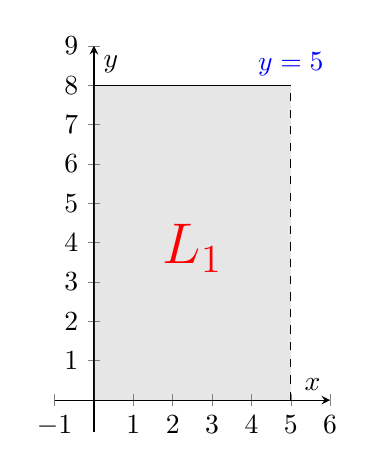
\begin{tikzpicture}
\begin{axis}[
x= 0.5 cm, y=0.5 cm,
 axis lines=middle,
  xmin=-1,xmax=6,ymin=-0.8,ymax=9,
  xtick distance=1,
  ytick distance=1,
  xlabel=$x$,
  ylabel=$y$]
\addplot [domain=0:5, name path=A] {8} node[above,blue] {$y=5$};
\addplot [domain=0:5, name path=B] {0};
\addplot[gray,opacity=0.2] fill between[of=B and A];
\draw[dashed] (5,0) -- (5,8);
\draw (2.5,3) node[red,above] {\huge{$L_1$}};
\end{axis}
\end{tikzpicture} \qquad
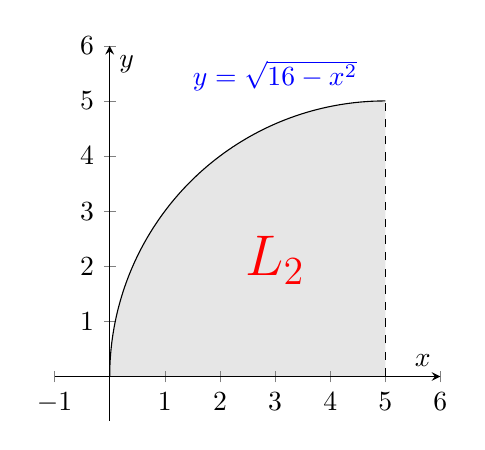
\begin{tikzpicture}
\begin{axis}[
x= 0.7 cm, y=0.7 cm,
 axis lines=middle,
  xmin=-1,xmax=6,ymin=-0.8,ymax=6,
  xtick distance=1,
  ytick distance=1,
  xlabel=$x$,
  ylabel=$y$]
\addplot [domain=0:5, name path=B,samples=3000] {sqrt(25-(x-5)^2)};
\addplot [domain=0:5, name path=A]{0};
\addplot[gray,opacity=0.2] fill between[of=B and A];
\draw (3,5) node[above,blue] {$y=\sqrt{16-x^2}$};
\draw (3,1.5) node[red, above] {\huge{$L_2$}};
\draw[dashed] (5,0) -- (5,5);
\end{axis}
\end{tikzpicture}
	 		\end{center}
	 		Mudah terlihat bahwa $L_1$ merupakan persegi panjang dengan panjang 8 dan lebar 5 sehingga $L_1=8\times 5=40$ dan $L_2$ merupakan seperempat lingkaran dengan jari-jari $5$ sehingga $L_2=\dfrac{1}{4}\pi(5)^2=\dfrac{25}{4}\pi$. Dapat diperoleh hasil integralnya adalah $L_1-L_2=40-\dfrac{25}{4}\pi$.
	\item Selesaikan integral berikut
	\begin{align*}
	\int \sqrt[3]{4x^2-20x+25}\, dx
	\end{align*}
	\textbf{Penyelesaian:}\\
	Tinjau bahwa $4x^2-20x+25=4\left(x^2-5x+\dfrac{25}{4}\right)=4\left(x-\frac{5}{2}\right)^2$ sehingga 
	\begin{align*}
	\int \sqrt[3]{4\left(x-\frac{5}{2}\right)^2}\, dx &= \int\sqrt[3]{4}\left(x-\frac{5}{2}\right)^{2/3} \, dx\\
	&=  \sqrt[3]{4}\left(x-\frac{5}{2}\right)^{5/3}\times \dfrac{1}{\frac{5}{3}}+C\\
	&= \dfrac{3\sqrt[3]{4}}{5}\left(x-\frac{5}{2}\right)^{5/3}+C
	\end{align*}
	\item Jika diberikan $\displaystyle F(x)=\int_2^x \dfrac{t^2-2t}{t^3-1}\, dt$ untuk $-\infty<x<\infty$, maka tentukan selang supaya $F$ naik dan $F$ turun.\\
	Untuk mencari selang naik atau turun, perlu dicari dulu $F'(x)$. Dengan menggunakan Teorema Fundamental Kalkulus II
	\begin{align*}
	F'(x) = \dfrac{x^2-2x}{x^3-1} = \dfrac{x(x-2)}{(x-1)(x^2+x+1)}
	\end{align*}
	Karena $x^2+x+1>0$, diperoleh pembuat nolnya adalah $x=0, x=1, x=2$. \\
	Didapatkan $F'(x)\leq 0$ pada selang $(-\infty,0]\cup (1,2]$ sehingga $F(x)$ turun pada selang tersebut. \\
	Didapatkan pula $F'(x)\geq 0$ pada selang $[0,1)\cup [2,+\infty)$ sehingga $F(x)$ naik pada selang tersebut.
	\item Jika $F(x)= \displaystyle \int_x^{x^2} \dfrac{t}{(3+t^2)^2}\, dt$, maka dapatkan $F(0), F(1),  F(-1), F'(-1)$. [Petunjuk: Gunakan Teorema Fundamental Kalkulus II]\\
	\textbf{Penyelesaian:}\\
	Ingat bahwa $\displaystyle \int_a^a f(x)\, dx=0$ sehingga 
	\begin{align*}
	F(0) &= \int_0^0 \dfrac{t}{(3+t^2)^2}\, dt = 0\\
	F(1) &= \int_1^1 \dfrac{t}{(3+t^2)^2}\, dt = 0
	\end{align*}
	Selanjutnya tinjau bahwa $f(t)=\dfrac{t}{(3+t^2)^2}$ adalah fungsi ganjil karena 
	\begin{align*}
	f(-t) = \dfrac{-t}{(3+(-t)^2)^2} = -\dfrac{t}{(3+t^2)^2} = -f(t)
	\end{align*}
	Ingat bahwa jika $f(x)$ fungsi ganjil, maka $\displaystyle \int_{-a}^a f(x)\, dx = 0$ sehingga 
	\begin{align*}
	F(-1) = \int_{-1}^1 \dfrac{t}{(3+t^2)^2} \, dt = 0
	\end{align*}
	Selanjutnya cari $F'(x)$ dengan Teorema Fundamental Kalkulus II dan aturan rantai, kita punya 
	\begin{align*}
	F'(x) &= \dfrac{x^2}{(3+(x^2)^2)^2}\dfrac{d}{dx}[x^2] - \dfrac{x}{(3+x^2)^2}\dfrac{d}{dx}[x] \\
	&= \dfrac{x^2}{(3+x^4)^2}-\dfrac{x}{(3+x^2)^2}
	\intertext{sehingga}
	F'(-1) &= \dfrac{(-1)^2}{(3+(-1)^4)^2} -\dfrac{-1}{(3+(-1)^2)^2}\\
	&= \dfrac{1}{16}+\dfrac{1}{16} = \dfrac{1}{8}
	\end{align*}
	\item Hitunglah integral berikut:
	\begin{align*}
	\int_{-5}^0 |2x+8|\, dx
\end{align*}	 
\textbf{Penyelesaian:}\\
Tinjau bahwa $|2x+8| = \begin{cases}2x+8, &x\geq -4\\
-2x-8, &x<-4\end{cases}$ sehingga integralnya menjadi 
\begin{align*}
\int_{-5}^0 |2x+8|\, dx &= \int_{-5}^{-4} -2x-8\, dx +\int_{-4}^0 2x+8\, dx\\
&= -x^2-8x\bigg|_{-5}^{-4} + x^2+8x\bigg|_{-4}^{0}\\
&= -16+32-(-25+40) + 0 - (16-32)\\
&= 17
\end{align*}
\item Diberikan $f(x)$ fungsi ganjil dengan $\displaystyle \int_0^2 f^2(x) \, dx=3$. Tentukan $$\displaystyle \int_{-2}^2 (\cos x) f(x) + (\sin x) f^4(x) + f^2(x) \, dx $$
\textbf{Penyelesaian:}\\
Perhatikan bahwa $\cos x$ fungsi genap karena $\cos (-x)=\cos (x)$, sedangkan $\sin x$ fungsi ganjil karena $\sin (-x) = -\sin x$. Selanjutnya, jika $f(x)$ fungsi ganjil dan $g(x)$ fungsi genap, maka 
\begin{align*}
f^2(-x) = f(-x)f(-x) = [-f(x)][-f(x)] &= f^2(x)\\
f^4(-x) = f^2(-x)f^2(-x) &= f^4(x)\\
f(-x)g(-x) &= -f(x)g(x)
\end{align*}
sehingga $f^2(x), f^4(x)$ fungsi genap dan $f(x)g(x)$ fungsi ganjil.\\
Didapatkan bahwa $(\cos x)f(x)$ fungsi ganjil serta $(\sin x)f^4(x)$ dan $f^2(x)$ fungsi genap.\\
Ingat bahwa untuk $f(x)$ fungsi ganjil dan $g(x)$ fungsi genap, berlaku
\begin{align*}
\int_{-a}^a f(x) = 0 \qquad \text{dan} \qquad
\int_{-a}^a g(x) = 2\int_0^a g(x)
\end{align*}
Didapatkan 
\begin{align*}
\int_{-2}^2 (\cos x) f(x) + (\sin x) f^4(x) + f^2(x) \, dx &= \int_{-2}^2 (\cos x) f(x) \, dx+ \int_{-2}^2 (\sin x) f^4(x) \, dx + \int_{-2}^2 f^2(x) \, dx\\
&= 0 + 0 + 2\int_0^2 f^2(x)\, dx\\
&= 2(3) = 6
\end{align*}
\item Hitunglah integral berikut 
\begin{align*}
\int \cos (4x)\sin (20x)\, dx
\end{align*}
\textbf{Penyelesaian:}\\
Ingat bahwa 
\begin{align*}
\sin (a+b) &= \sin a\cos b+\cos a\sin b\\
\sin(a-b) &= \sin a\cos b -\cos a\sin b
\end{align*}
sehingga $\cos a \sin b = \dfrac{1}{2}[\sin (a+b)-\sin(a-b)]$. Didapatkan 
\begin{align*}
\cos (4x)\sin (20x) = \dfrac{1}{2}[\sin (24x) - \sin (-16x)] = \dfrac{1}{2}[\sin (24x) +\sin (16x)]
\end{align*}
Selanjutnya ingat bahwa 
\begin{align*}
\int \sin (ax) \, dx = -\dfrac{1}{a}\cos (ax) + C
\end{align*}
untuk suatu $a\neq 0$. Dari sini, diperoleh 
\begin{align*}
\int \cos (4x)\sin (20x)\, dx &= \int \dfrac{1}{2}[\sin (24x) +\sin (16x)]\, dx \\
&= \dfrac{1}{2}\left[ -\dfrac{1}{24}\cos (24x) - \dfrac{1}{16}\cos (16x)\right] + C\\
&= -\dfrac{1}{48}\cos (24x) - \dfrac{1}{32} \cos (16x) + C
\end{align*}
\end{enumerate}
\end{document}
 
